\section{Experiments}
\label{sec:exp}

\noindent\textbf{Datasets and protocol.} We use Mip-NeRF~360~\cite{barron2022mipnerf360} (9 scenes), Tanks and Temples~\cite{knapitsch2017tanks} (truck, train), Deep Blending~\cite{hedman2018deep} (drjohnson, playroom) and NeRF-Synthetic~\cite{mildenhall2020nerf} (8 objects), 21 scenes in total. The training settings of \MS are unchanged: 30k iterations, images downsampled by 2 indoors and by 4 outdoors, the standard test split, and a black background for NeRF-Synthetic. Quality is the PSNR, SSIM and LPIPS of the \emph{decoded file}. Every size is the size of the single file that the encoder writes. The \emph{FP32 model} is the mesh that \MS produces with its released settings, stored in 32-bit floats (our reproduction).

\noindent\textbf{Settings.} The controller uses one setting for all 21 scenes and all target sizes: the file is measured every 500 iterations from 12.5k to 29.5k, and growth aims at 1.35 times the target. The codec uses codebooks of 4{,}096 and 256 entries and 7 bits for the DC color everywhere. Positions use 14 to 18 bits depending on the scene (14 for the objects, 14--16 for Mip-NeRF~360, 15 for Deep Blending, 18 for Tanks and Temples). Every baseline on a scene uses the same position precision as \BM.

\noindent\textbf{Baselines.} No codec exists for these meshes, so we build the baselines from what is available. For the mesh, \MS has no size control; its cap on the number of vertices is the only parameter that affects the size, so we lower the cap to obtain smaller meshes. We also simplify the constructed FP32 model by edge collapse. For the file, we use three generic mesh codecs: TFAN~\cite{mamou2009tfan}, Draco~\cite{draco} and a quantized PLY compressed with zstd. Each generic codec is run with the SH coefficients quantized to 8, 6 and 4 bits, and we keep its best points. We summarize curves by BD-PSNR and BD-rate, computed with piecewise-linear interpolation over the logarithm of the file size.

%------------------------------------------------------------------
\begin{figure*}[t]\centering
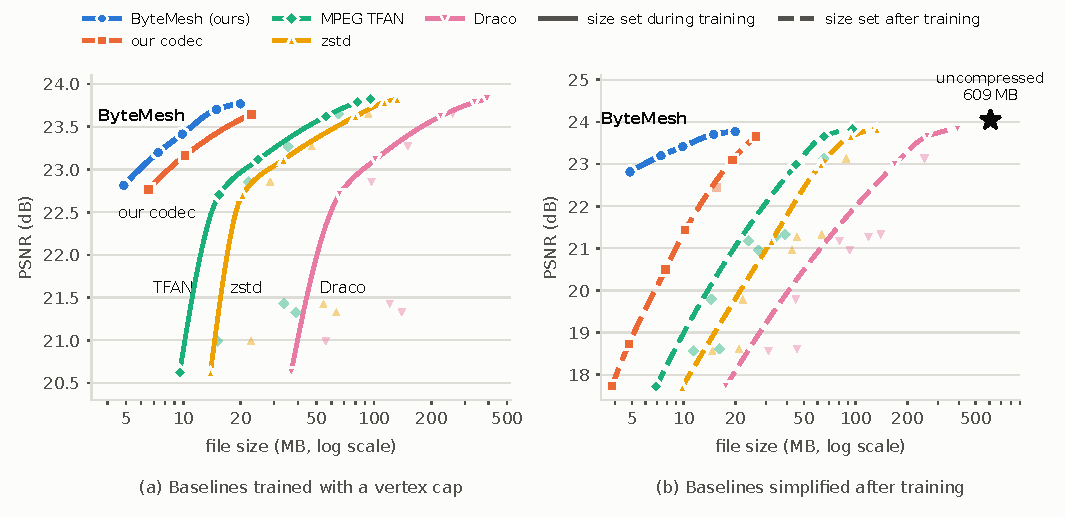
\includegraphics[width=\linewidth]{figures/fig_rd_pair_v4.pdf}
\caption{\textbf{Rate--distortion on Mip-NeRF~360 and Tanks and Temples} (mean over 11 scenes). (a)~Baselines trained with a vertex cap and written with our codec or a generic codec. (b)~Baselines obtained by simplifying the FP32 model (star, 609~MB) after training. \BM is the same curve in both panels; the two panels have different PSNR axes.}
\label{fig:rd}
\end{figure*}

%------------------------------------------------------------------

\subsection{Rate--distortion against the baselines}
\label{sec:rd}
Fig.~\ref{fig:rd} compares \BM with every baseline on the 11 scenes of Mip-NeRF~360 and Tanks and Temples. \BM gives 22.81\dB at 4.9~MB and 23.77\dB at 19.9~MB. The FP32 model gives 24.05\dB at 609~MB, so the files are 31, 62 and 125 times smaller at 20, 10 and 5~MB, for a loss of 0.28, 0.64 and 1.24\dB. The same comparison in SSIM and LPIPS is in the supplement and gives the same order of the methods.

\noindent\textbf{Vertex cap with a generic codec (Fig.~\ref{fig:rd}a).} In BD-rate, \BM needs 75\% fewer bytes than the cap with TFAN, 82\% fewer than with zstd and 94\% fewer than with Draco (Table~\ref{tab:bd}). Read at the five target sizes, to reach the PSNR of \BM TFAN needs files 3.6--4.5$\times$ larger, zstd 4.8--6.4$\times$ larger and Draco 15--18$\times$ larger, over the five target sizes. On the eight objects the factors are 1.7--2.1$\times$, 2.1--2.7$\times$ and 8.6--11$\times$ (supplement). The factors are smaller there because the files are only 1.5 to 4~MB and the codebooks are a fixed cost.

\noindent\textbf{Vertex cap with our codec (Fig.~\ref{fig:rd}a).} This baseline isolates the effect of the controller, because the codec is the same. Table~\ref{tab:bd} gives the Bjontegaard deltas. \BM is better on 20 of the 21 scenes and equal on one (treehill): the BD-PSNR is $+0.29$\dB on average and the BD-rate is $-26.9\%$.

\noindent\textbf{Simplification after training (Fig.~\ref{fig:rd}b).} Simplifying the FP32 model loses more quality the further the mesh is reduced. Against \BM at the same file size, the simplified mesh is 0.3--2.1\dB worse at 12--19~MB, 1.0--3.6\dB worse at 8--12~MB and 1.8--5.9\dB worse below 8~MB (45 matched points on 11 scenes, same codec). The reason is that each pixel is covered by one opaque triangle: after a collapse, the neighboring triangles have not been trained for their new shape, and no other primitive covers the error.

\begin{table}[t]\centering\footnotesize
\caption{\textbf{Bjontegaard deltas of \BM} against each baseline, computed per scene and averaged. Negative BD-rate: \BM needs fewer bytes for the same PSNR. Draco has no file size in common with \BM, so its BD-PSNR is undefined.}
\label{tab:bd}
\setlength{\tabcolsep}{4pt}
\begin{tabular}{@{}llcc@{}}
\toprule
baseline & scenes & BD-PSNR & BD-rate \\
\midrule
\multicolumn{4}{@{}l}{\emph{Vertex cap + our codec}} \\
 & Mip-NeRF 360, T\&T (11) & $+0.30$ dB & $-31.3\%$ \\
 & Deep Blending (2) & $+0.23$ dB & $-22.8\%$ \\
 & NeRF-Synthetic (8) & $+0.29$ dB & $-21.1\%$ \\
 & all (21) & $+0.29$ dB & $-26.9\%$ \\
\midrule
\multicolumn{4}{@{}l}{\emph{Vertex cap + generic codec}} \\
TFAN & Mip-NeRF 360, T\&T (11) & $+1.90$ dB & $-75.3\%$ \\
zstd & Mip-NeRF 360, T\&T (11) & $+2.50$ dB & $-81.9\%$ \\
Draco & Mip-NeRF 360, T\&T (11) & -- & $-94.1\%$ \\
\bottomrule
\end{tabular}
\end{table}

\subsection{The codec alone}
\label{sec:codec}
Here every codec encodes the \emph{same} mesh, so the mesh plays no role. The meshes are trained with vertex caps of 0.6, 1.08 and 3 million. For each scene we find the file size at which a generic codec reaches the PSNR of our file. On Mip-NeRF~360 and Tanks and Temples, TFAN needs 2.5--2.8$\times$ the size of our file, zstd 3.4--4.0$\times$ and Draco about 11$\times$. On the objects the factors are 1.4--1.8$\times$, 1.8--2.3$\times$ and 7.6--9.1$\times$. The lossy steps of the codec (vector quantization of the SH coefficients and quantization of positions and color) lower the PSNR by 0.15, 0.20 and 0.27\dB on average on the three meshes, and by at most 0.63\dB on one scene. At 10~MB on garden, the file holds connectivity (39\%), positions (21\%), SH indices (19\%), DC color (15\%) and the codebooks (7\%).

\begin{table}[t]\centering\footnotesize
\caption{\textbf{Encoding and decoding time} in seconds, mean over 11 scenes (about 0.93 million vertices each), CPU only. TFAN is called once for both directions.}
\label{tab:time}
\begin{tabular}{@{}lcc@{}}
\toprule
codec & encode & decode \\
\midrule
zstd (quantized PLY) & 15.4 & 0.2 \\
Draco & 16.6 & 3.8 \\
TFAN & \multicolumn{2}{c}{8.2 (both)} \\
\BM & 4.6 & 3.7 \\
\bottomrule
\end{tabular}
\end{table}

\noindent\textbf{Time.} Table~\ref{tab:time} gives the encoding and decoding times. Our encoder takes 4.6~s and our decoder 3.7~s for a mesh of about 0.93 million vertices. Building the codebooks before encoding takes 1.5 minutes on a GPU, for \BM and for the cap baseline alike.

\subsection{Controlling the file size}
\label{sec:control}

\begin{table}[t]\centering\footnotesize
\caption{\textbf{\BM at each target size}, dataset means over single runs. Size error is $|\text{file}-\text{target}|/\text{target}$. $^\dagger$Two objects (ficus, mic) are fully represented by about 2 to 2.6~MB and do not grow further.}
\label{tab:main}
\setlength{\tabcolsep}{3.2pt}
\begin{tabular}{@{}llccccc@{}}
\toprule
dataset & target & file & size err. & PSNR & SSIM & LPIPS \\
\midrule
\multirow{5}{*}{\shortstack[l]{Mip-NeRF\\360 (9)}} & 20 MB & 19.91 & 0.8\% & 24.46 & 0.707 & 0.406 \\
 & 15 MB & 14.92 & 0.7\% & 24.38 & 0.698 & 0.423 \\
 & 10 MB & 9.87 & 1.5\% & 24.06 & 0.678 & 0.453 \\
 & 7.5 MB & 7.35 & 2.0\% & 23.83 & 0.661 & 0.475 \\
 & 5 MB & 4.85 & 2.9\% & 23.42 & 0.635 & 0.506 \\
\midrule
\multirow{5}{*}{\shortstack[l]{Tanks and\\Temples (2)}} & 20 MB & 20.01 & 0.2\% & 20.64 & 0.750 & 0.332 \\
 & 15 MB & 15.02 & 0.1\% & 20.67 & 0.747 & 0.341 \\
 & 10 MB & 9.94 & 0.6\% & 20.51 & 0.736 & 0.361 \\
 & 7.5 MB & 7.45 & 0.7\% & 20.36 & 0.722 & 0.381 \\
 & 5 MB & 4.96 & 0.8\% & 20.09 & 0.703 & 0.408 \\
\midrule
\multirow{5}{*}{\shortstack[l]{Deep\\Blending (2)}} & 20 MB & 19.93 & 0.9\% & 27.01 & 0.840 & 0.450 \\
 & 15 MB & 14.82 & 1.2\% & 26.84 & 0.839 & 0.459 \\
 & 10 MB & 9.93 & 0.7\% & 26.69 & 0.833 & 0.474 \\
 & 7.5 MB & 7.30 & 2.6\% & 26.40 & 0.829 & 0.485 \\
 & 5 MB & 4.99 & 0.3\% & 26.04 & 0.821 & 0.498 \\
\midrule
\multirow{3}{*}{\shortstack[l]{NeRF-\\Synthetic (8)}} & 4 MB$^\dagger$ & 3.56 & 11.3\% & 31.20 & 0.952 & 0.069 \\
 & 2.5 MB$^\dagger$ & 2.43 & 3.2\% & 31.10 & 0.951 & 0.069 \\
 & 1.5 MB & 1.50 & 0.3\% & 30.45 & 0.945 & 0.079 \\
\bottomrule
\end{tabular}
\end{table}

\begin{figure}[t]\centering
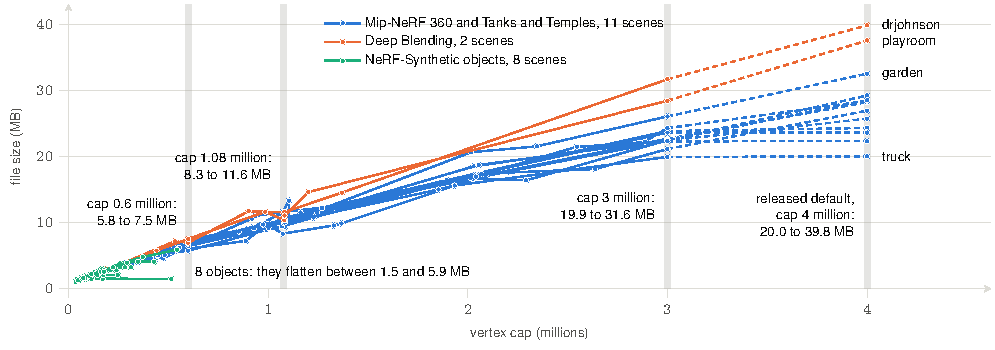
\includegraphics[width=\linewidth]{figures/fig_cap_instability.pdf}
\caption{\textbf{File size against the vertex cap}, one line per scene, same codec. Dashed segments lead to the released default of 4 million. The numbers on top give the range of file sizes over the captured scenes at four caps. The same cap gives different file sizes on different scenes, and the spread grows with the cap.}
\label{fig:cap}
\end{figure}

\noindent\textbf{A vertex cap does not set the file size.} Fig.~\ref{fig:cap} plots the file size against the cap for every scene. With the same cap, the captured scenes give files of 5.8--7.5~MB at 0.6 million vertices, 8.3--11.6~MB at 1.08 million, 19.9--31.6~MB at 3 million and 20.0--39.8~MB at the default 4 million: the largest file is 1.3 to 2.0 times the smallest. Some scenes stop growing before the cap (truck, train and counter give the same file at 3 and 4 million). A user therefore cannot choose the cap for a given file size without first training the scene. Even with all our runs in hand, the best single curve from cap to file size misses by more than 10\% in 68 of 191 cap runs.

\noindent\textbf{\BM takes the file size as its input.} Table~\ref{tab:main} lists the file size and the quality of \BM at every target on the four datasets, from single runs. On the captured scenes the mean error is at most 2.9\% for every dataset and target, and all 65 runs end within 10\% of the target. On the objects, 21 of 24 runs end within 10\%. The three others are ficus and mic at 2.5 or 4~MB: these objects are fully represented by about 2 to 2.6~MB, the controller finds no more triangles with an error to split, and the file stays below the target.

\noindent\textbf{Training time.} One run of \BM takes 48.8 minutes on average on the 13 captured scenes (one L40S GPU), against 28.0 minutes for one run of \MS with a cap. A cap user who does not know the scene needs a first run with the default settings to see its size, and then at least one capped run. Counted this way, the cap took 82.4 minutes on average to come within 10\% of a 10~MB target, against 54.7 minutes for \BM, both including a fine-tuning stage that we report in the supplement.

\subsection{Other representations}
\label{sec:cross}

\begin{table*}[t]\centering\footnotesize
\caption{\textbf{Other representations}, dataset means; size in MB. Gaussian rows are published numbers collected in~\cite{hacpp2025} and are given for reference: they are a different representation. Mesh rows in (a) are published numbers collected in~\cite{meshsplatting2025}; n/r: not reported. \MS FP32 is our reproduction. $^\ddagger$Rendered on a black background.}
\label{tab:cross}
\setlength{\tabcolsep}{2.6pt}
\begin{tabular}[t]{@{}c@{}}\textbf{(a)} Mip-NeRF 360 and Tanks and Temples\\[2pt]
\begin{tabular}[t]{@{}lcccccccc@{}}
\toprule
 & \multicolumn{4}{c}{Mip-NeRF 360} & \multicolumn{4}{c}{Tanks and Temples} \\
\cmidrule(lr){2-5}\cmidrule(lr){6-9}
method & PSNR & SSIM & LPIPS & MB & PSNR & SSIM & LPIPS & MB \\
\midrule
3DGS~\cite{kerbl2023gaussians} & 27.46 & 0.812 & 0.222 & 750.9 & 23.69 & 0.844 & 0.178 & 431.0 \\
Compact3DGS~\cite{compact3dgs2024} & 27.08 & 0.798 & 0.247 & 48.80 & 23.32 & 0.831 & 0.201 & 39.43 \\
HAC++~\cite{hacpp2025}, low & 27.60 & 0.803 & 0.253 & 8.34 & 24.22 & 0.849 & 0.190 & 5.18 \\
HAC++, high & 27.82 & 0.811 & 0.231 & 18.48 & 24.32 & 0.854 & 0.178 & 8.63 \\
\midrule
GOF mesh~\cite{gof2024} & 20.78 & 0.573 & 0.465 & 1500 & 21.69 & 0.690 & 0.326 & n/r \\
RaDe-GS mesh~\cite{rade2024} & 23.56 & 0.668 & 0.361 & 1100 & 20.51 & 0.659 & 0.344 & n/r \\
MiLo~\cite{milo2025} & 24.09 & 0.688 & 0.323 & 253 & 21.46 & 0.706 & 0.348 & n/r \\
\MS FP32~\cite{meshsplatting2025} & 24.81 & 0.731 & 0.309 & 642 & 20.64 & 0.760 & 0.272 & 459 \\
\midrule
\BM, 20 MB & 24.46 & 0.707 & 0.406 & 19.9 & 20.64 & 0.750 & 0.332 & 20.0 \\
\BM, 10 MB & 24.06 & 0.678 & 0.453 & 9.9 & 20.51 & 0.736 & 0.361 & 9.9 \\
\BM, 5 MB & 23.42 & 0.635 & 0.506 & 4.9 & 20.09 & 0.703 & 0.408 & 5.0 \\
\bottomrule
\end{tabular}
\end{tabular}\hfill
\begin{tabular}[t]{@{}c@{}}\textbf{(b)} NeRF-Synthetic\\[2pt]
\begin{tabular}[t]{@{}lcccc@{}}
\toprule
 & \multicolumn{4}{c}{8 objects} \\
\cmidrule(lr){2-5}
method & PSNR & SSIM & LPIPS & MB \\
\midrule
3DGS~\cite{kerbl2023gaussians} & 33.80 & 0.970 & 0.031 & 68.46 \\
Compact3DGS~\cite{compact3dgs2024} & 33.33 & 0.968 & 0.034 & 5.54 \\
HAC++~\cite{hacpp2025}, low & 33.03 & 0.966 & 0.039 & 0.88 \\
HAC++, high & 33.76 & 0.969 & 0.033 & 1.84 \\
\midrule
MobileNeRF~\cite{mobilenerf2023} & 30.90 & 0.947 & 0.062 & 125.8 \\
NeRF2Mesh~\cite{nerf2mesh2023} & 29.76 & 0.940 & 0.072 & 73.5 \\
\MS FP32$^\ddagger$ & 31.17 & 0.955 & 0.063 & 65.7 \\
\midrule
\BM$^\ddagger$, 4 MB & 31.20 & 0.952 & 0.069 & 3.56 \\
\BM$^\ddagger$, 2.5 MB & 31.10 & 0.951 & 0.069 & 2.43 \\
\BM$^\ddagger$, 1.5 MB & 30.45 & 0.945 & 0.079 & 1.50 \\
\bottomrule
\end{tabular}
\end{tabular}
\end{table*}

Table~\ref{tab:cross} places \BM among other representations. Among the methods that output a mesh, \BM is the only one below 250~MB. At 20~MB it is 0.35\dB below the FP32 model of \MS on Mip-NeRF~360 and equal to it on Tanks and Temples, and it is above MiLo, RaDe-GS and GOF on Mip-NeRF~360 with files 13 to 75 times smaller. On NeRF-Synthetic, the 3.6~MB file matches the PSNR of the 65.7~MB FP32 model (31.20 against 31.17\dB), with slightly lower SSIM and higher LPIPS, and the 2.5~MB file has a higher PSNR than MobileNeRF and NeRF2Mesh at about 1/50 and 1/30 of their size.

Compressed Gaussians remain better at the same size: HAC++ is 3.4 to 4.2\dB higher in PSNR on the captured scenes. This gap comes from the representation (opaque triangles against semi-transparent Gaussians) and is already present before compression, between \MS and 3DGS. What the mesh offers in exchange is a standard indexed triangle mesh that any engine renders without sorting. In a WebGL viewer on a laptop (Apple M2 Max, $1920 \times 958$), the 5, 10 and 20~MB files of garden, room and bicycle render in 1.1, 1.3 and 2.0~ms per frame on average (about 960, 760 and 500 frames per second).

\subsection{Ablation}
\label{sec:abl}

\begin{table}[t]\centering\footnotesize
\caption{\textbf{Selection rules}, PSNR at a target of 10~MB, one run each. ``Importance'' is the score that \MS uses for its own densification. Every file is within 1\% of the target.}
\label{tab:abl}
\setlength{\tabcolsep}{4pt}
\begin{tabular}{@{}lcc@{}}
\toprule
 & garden & room \\
\midrule
\BM & 23.67 & 27.99 \\
split by importance & 23.51 ($-0.17$) & 27.56 ($-0.43$) \\
collapse by importance & 22.89 ($-0.78$) & 25.61 ($-2.38$) \\
\bottomrule
\end{tabular}
\end{table}

\noindent\textbf{Selection rules.} \BM chooses the triangles to split by their accumulated rendering error, and the edges to collapse by the rendering error per byte saved. Table~\ref{tab:abl} replaces each rule in turn by the importance score of \MS and keeps everything else. The split rule accounts for 0.17 and 0.43\dB, and the collapse rule for 0.78 and 2.38\dB, at the same file size. The collapse rule matters more because vertices are removed in up to 35 rounds, and a poor choice is repeated in each of them.

\noindent\textbf{Collapse schedule.} \BM measures the file every 500 iterations until 29.5k and removes the measured excess each time. We compare it with a variant that stops the collapse rounds at 19.5k and predicts the final file size from the measurements up to then. On the 33 runs of Mip-NeRF~360 and Tanks and Temples, the mean size error falls from 4.3\% to 1.5\%, and the number of runs within 2\% of the target rises from 7 to 23. At the same file size, the PSNR is higher by 0.02, 0.06 and 0.13\dB at 20, 10 and 5~MB. On Deep Blending the size error falls from 5.8--9.8\% to 0.3--0.9\%. Measuring until the end is both more accurate and slightly better in quality than predicting.

\begin{table}[t]\centering\footnotesize
\caption{\textbf{Growth aim $\alpha$}, target 10~MB, one run each. File size in MB and PSNR in dB. \BM uses $\alpha = 1.35$.}
\label{tab:alpha}
\setlength{\tabcolsep}{5pt}
\begin{tabular}{@{}lcccc@{}}
\toprule
 & \multicolumn{2}{c}{garden} & \multicolumn{2}{c}{room} \\
\cmidrule(lr){2-3}\cmidrule(lr){4-5}
$\alpha$ & file & PSNR & file & PSNR \\
\midrule
1.0 & 8.46 & 23.33 & 8.72 & 27.65 \\
1.2 & 9.94 & 23.57 & 10.03 & 27.90 \\
1.35 & 10.00 & 23.67 & 9.99 & 27.99 \\
1.5 & 9.96 & 23.76 & 9.70 & 27.84 \\
\bottomrule
\end{tabular}
\end{table}

\noindent\textbf{Growth aim.} \BM grows the mesh to $\alpha = 1.35$ times the target and then removes the excess. Table~\ref{tab:alpha} varies $\alpha$. With $\alpha = 1.0$, the file ends 13\% to 15\% below the target and no collapse round is active: vertices are lost between the end of densification and the final mesh, and nothing can add them back. Growing past the target is therefore necessary. Between 1.2 and 1.5, the file is on target and the PSNR changes by less than 0.2\dB; garden improves with a larger $\alpha$ and room is best at 1.35. We use 1.35 for all scenes.

\begin{table}[t]\centering\footnotesize
\caption{\textbf{Codec design choices}, bits per vertex, mean over 11 scenes (meshes of about one million vertices). Every stream was decoded and checked. The first row of each block is the codec used for all results; ``file'' is the change in file size against it.}
\label{tab:codec-abl}
\setlength{\tabcolsep}{4pt}
\begin{tabular}{@{}llcc@{}}
\toprule
stream & variant & bits & file \\
\midrule
\multirow{4}{*}{positions} & one earlier neighbor & 22.6 & -- \\
 & previous vertex & 23.2 & $+0.7\%$ \\
 & parallelogram & 23.5 & $+1.0\%$ \\
 & mean of earlier neighbors & 21.6 & $-1.1\%$ \\
\midrule
\multirow{2}{*}{DC color} & zstd, no prediction & 12.6 & -- \\
 & mean of earlier neighbors & 11.3 & $-1.5\%$ \\
\midrule
\multirow{3}{*}{SH indices} & neighbor candidates & 17.6 & -- \\
 & no neighbor information & 17.4 & $-0.3\%$ \\
 & fixed length & 20.0 & $+2.8\%$ \\
\bottomrule
\end{tabular}
\end{table}

\noindent\textbf{Codec design choices.} Table~\ref{tab:codec-abl} measures alternatives for three streams on the same meshes. For positions, predicting from one earlier neighbor is better than the previous vertex and than parallelogram prediction on all 11 scenes; the parallelogram is the worst because many edges of these meshes are boundary edges. Predicting from the mean of all earlier neighbors is better still, and the same holds for the DC color. For the SH indices, offering the indices of the neighbors as candidates does not help: an adaptive model without neighbor information gives slightly smaller streams. Neighboring vertices rarely share a codeword, and the saving over fixed-length codes comes from the uneven use of the codewords. Together, the better variants would make the files about 2.9\% smaller. They are not used in any reported file size, so the sizes in this paper are conservative. The size of the two codebooks is studied in the supplement: choosing the best size per scene and per file size would gain at most 0.15\dB over the fixed choice.

\noindent\textbf{Limitations.} LPIPS degrades more than PSNR: on Mip-NeRF~360 it rises from 0.309 for the FP32 model to 0.406 at 20~MB and 0.506 at 5~MB. Training does not see the vector quantization: the per-triangle error is measured on the unquantized mesh, and the codebooks are fitted after training. The position precision is set per scene and is not chosen by the controller. An object that is fully represented below the target stays below it. The ablations of the selection rules and of the growth aim use two scenes and one run each.

%==================================================================
% SUPPLEMENT (paste into the appendix file)
%==================================================================
% \begin{figure*}[t]\centering
% 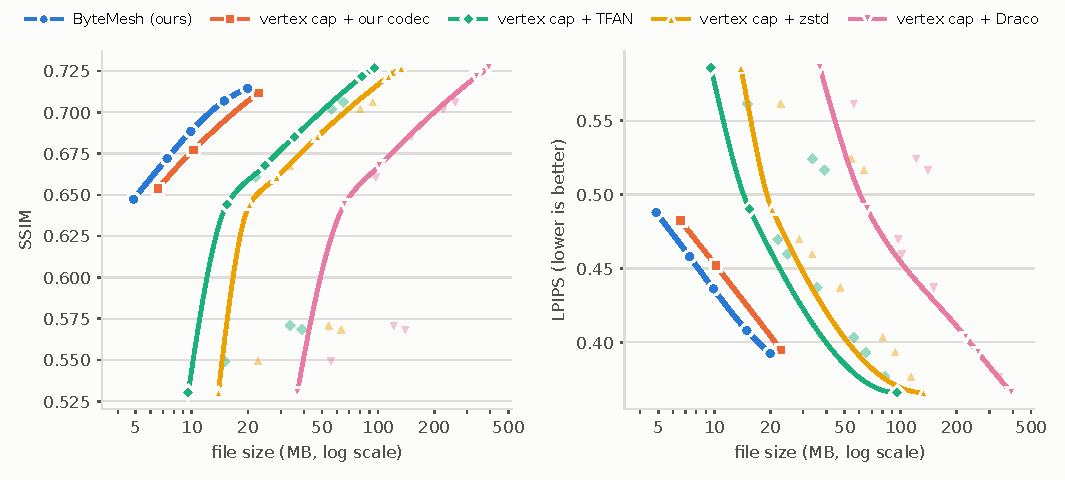
\includegraphics[width=\linewidth]{figures/fig_rd_ssim_lpips_v2.pdf}
% \caption{\textbf{SSIM and LPIPS against file size} on Mip-NeRF~360 and Tanks and Temples (mean over 11 scenes), for the baselines trained with a vertex cap. Same runs as Fig.~\ref{fig:rd}a.}
% \label{fig:rd-ssim-lpips}
% \end{figure*}
%
% \begin{figure}[t]\centering
% 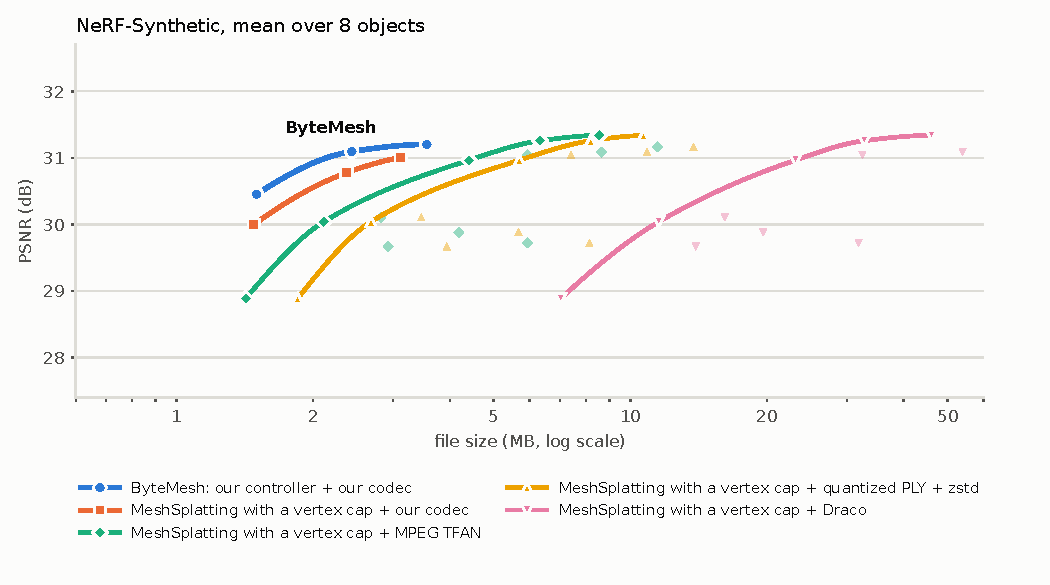
\includegraphics[width=\linewidth]{figures/fig_rd_objects_v3.pdf}
% \caption{\textbf{Rate--distortion on NeRF-Synthetic} (mean over 8 objects), baselines trained with a vertex cap.}
% \label{fig:rd-objects}
% \end{figure}
%
% \noindent\textbf{Codebook size.} Table~\ref{tab:kr} compares five sizes of the two codebooks on the 11 scenes of Mip-NeRF~360 and Tanks and Temples at four file sizes. Removing the residual codebook saves about 8\% of the bytes and loses 0.12 to 0.15\dB. Enlarging the codebooks to 16{,}384 and 1{,}024 makes the files 12\% to 49\% larger for a gain of 0.06 to 0.07\dB. If the best size were chosen for each scene and each file size, the gain over the fixed choice would be between 0.02 and 0.15\dB per scene (0.08\dB on average); the largest gains are at the smallest files, where 1{,}024 + 256 is more efficient. The sweep was run on meshes from an earlier version of our training; the codec is the same.
%
% \begin{table*}[t]\centering\footnotesize
% \caption{\textbf{Codebook size.} Change in file size and PSNR (dB) against $K{=}4{,}096$, $K_r{=}256$, mean over 11 scenes, at four file sizes (size of the default file in the header).}
% \label{tab:kr}
% \begin{tabular}{@{}lcccc@{}}
% \toprule
% $K + K_r$ & 4.5 MB & 9.4 MB & 20.4 MB & 27.0 MB \\
% \midrule
% 4{,}096 + 0 & $-8.0\%$, $-0.12$ & $-8.4\%$, $-0.14$ & $-8.7\%$, $-0.15$ & $-8.9\%$, $-0.15$ \\
% 1{,}024 + 256 & $-12.8\%$, $-0.05$ & $-7.6\%$, $-0.05$ & $-5.0\%$, $-0.07$ & $-4.4\%$, $-0.07$ \\
% 4{,}096 + 256 & \multicolumn{4}{c}{reference} \\
% 4{,}096 + 1{,}024 & $+4.4\%$, $+0.02$ & $+3.3\%$, $+0.02$ & $+2.7\%$, $+0.03$ & $+2.7\%$, $+0.03$ \\
% 16{,}384 + 1{,}024 & $+49\%$, $+0.06$ & $+27\%$, $+0.06$ & $+15\%$, $+0.07$ & $+12\%$, $+0.07$ \\
% \bottomrule
% \end{tabular}
% \end{table*}
%
% \noindent\textbf{Prediction of the DC color.} In the codec used for all results, the DC color is quantized to 7 bits and compressed with zstd. We also coded it with a prediction from the vertices decoded earlier (the rounded mean of the earlier neighbors) and a context-adaptive binary arithmetic coder, and verified an exact round trip. On the 11 scenes of Mip-NeRF~360 and Tanks and Temples, the DC stream goes from 12.6 to 11.3 bits per vertex ($-10.4\%$) and the file becomes 1.46\% smaller on average ($0.84\%$ to $2.00\%$). The reported file sizes do not include this gain.
